% Options for packages loaded elsewhere
\PassOptionsToPackage{unicode}{hyperref}
\PassOptionsToPackage{hyphens}{url}
%
\documentclass[
]{article}
\title{MA7007 - Statistical Modelling and Forecasting Case Study Report
2023-2024}
\author{}
\date{\vspace{-2.5em}}

\usepackage{amsmath,amssymb}
\usepackage{lmodern}
\usepackage{iftex}
\ifPDFTeX
  \usepackage[T1]{fontenc}
  \usepackage[utf8]{inputenc}
  \usepackage{textcomp} % provide euro and other symbols
\else % if luatex or xetex
  \usepackage{unicode-math}
  \defaultfontfeatures{Scale=MatchLowercase}
  \defaultfontfeatures[\rmfamily]{Ligatures=TeX,Scale=1}
\fi
% Use upquote if available, for straight quotes in verbatim environments
\IfFileExists{upquote.sty}{\usepackage{upquote}}{}
\IfFileExists{microtype.sty}{% use microtype if available
  \usepackage[]{microtype}
  \UseMicrotypeSet[protrusion]{basicmath} % disable protrusion for tt fonts
}{}
\makeatletter
\@ifundefined{KOMAClassName}{% if non-KOMA class
  \IfFileExists{parskip.sty}{%
    \usepackage{parskip}
  }{% else
    \setlength{\parindent}{0pt}
    \setlength{\parskip}{6pt plus 2pt minus 1pt}}
}{% if KOMA class
  \KOMAoptions{parskip=half}}
\makeatother
\usepackage{xcolor}
\IfFileExists{xurl.sty}{\usepackage{xurl}}{} % add URL line breaks if available
\IfFileExists{bookmark.sty}{\usepackage{bookmark}}{\usepackage{hyperref}}
\hypersetup{
  pdftitle={MA7007 - Statistical Modelling and Forecasting Case Study Report 2023-2024},
  hidelinks,
  pdfcreator={LaTeX via pandoc}}
\urlstyle{same} % disable monospaced font for URLs
\usepackage[margin=1in]{geometry}
\usepackage{color}
\usepackage{fancyvrb}
\newcommand{\VerbBar}{|}
\newcommand{\VERB}{\Verb[commandchars=\\\{\}]}
\DefineVerbatimEnvironment{Highlighting}{Verbatim}{commandchars=\\\{\}}
% Add ',fontsize=\small' for more characters per line
\usepackage{framed}
\definecolor{shadecolor}{RGB}{248,248,248}
\newenvironment{Shaded}{\begin{snugshade}}{\end{snugshade}}
\newcommand{\AlertTok}[1]{\textcolor[rgb]{0.94,0.16,0.16}{#1}}
\newcommand{\AnnotationTok}[1]{\textcolor[rgb]{0.56,0.35,0.01}{\textbf{\textit{#1}}}}
\newcommand{\AttributeTok}[1]{\textcolor[rgb]{0.77,0.63,0.00}{#1}}
\newcommand{\BaseNTok}[1]{\textcolor[rgb]{0.00,0.00,0.81}{#1}}
\newcommand{\BuiltInTok}[1]{#1}
\newcommand{\CharTok}[1]{\textcolor[rgb]{0.31,0.60,0.02}{#1}}
\newcommand{\CommentTok}[1]{\textcolor[rgb]{0.56,0.35,0.01}{\textit{#1}}}
\newcommand{\CommentVarTok}[1]{\textcolor[rgb]{0.56,0.35,0.01}{\textbf{\textit{#1}}}}
\newcommand{\ConstantTok}[1]{\textcolor[rgb]{0.00,0.00,0.00}{#1}}
\newcommand{\ControlFlowTok}[1]{\textcolor[rgb]{0.13,0.29,0.53}{\textbf{#1}}}
\newcommand{\DataTypeTok}[1]{\textcolor[rgb]{0.13,0.29,0.53}{#1}}
\newcommand{\DecValTok}[1]{\textcolor[rgb]{0.00,0.00,0.81}{#1}}
\newcommand{\DocumentationTok}[1]{\textcolor[rgb]{0.56,0.35,0.01}{\textbf{\textit{#1}}}}
\newcommand{\ErrorTok}[1]{\textcolor[rgb]{0.64,0.00,0.00}{\textbf{#1}}}
\newcommand{\ExtensionTok}[1]{#1}
\newcommand{\FloatTok}[1]{\textcolor[rgb]{0.00,0.00,0.81}{#1}}
\newcommand{\FunctionTok}[1]{\textcolor[rgb]{0.00,0.00,0.00}{#1}}
\newcommand{\ImportTok}[1]{#1}
\newcommand{\InformationTok}[1]{\textcolor[rgb]{0.56,0.35,0.01}{\textbf{\textit{#1}}}}
\newcommand{\KeywordTok}[1]{\textcolor[rgb]{0.13,0.29,0.53}{\textbf{#1}}}
\newcommand{\NormalTok}[1]{#1}
\newcommand{\OperatorTok}[1]{\textcolor[rgb]{0.81,0.36,0.00}{\textbf{#1}}}
\newcommand{\OtherTok}[1]{\textcolor[rgb]{0.56,0.35,0.01}{#1}}
\newcommand{\PreprocessorTok}[1]{\textcolor[rgb]{0.56,0.35,0.01}{\textit{#1}}}
\newcommand{\RegionMarkerTok}[1]{#1}
\newcommand{\SpecialCharTok}[1]{\textcolor[rgb]{0.00,0.00,0.00}{#1}}
\newcommand{\SpecialStringTok}[1]{\textcolor[rgb]{0.31,0.60,0.02}{#1}}
\newcommand{\StringTok}[1]{\textcolor[rgb]{0.31,0.60,0.02}{#1}}
\newcommand{\VariableTok}[1]{\textcolor[rgb]{0.00,0.00,0.00}{#1}}
\newcommand{\VerbatimStringTok}[1]{\textcolor[rgb]{0.31,0.60,0.02}{#1}}
\newcommand{\WarningTok}[1]{\textcolor[rgb]{0.56,0.35,0.01}{\textbf{\textit{#1}}}}
\usepackage{graphicx}
\makeatletter
\def\maxwidth{\ifdim\Gin@nat@width>\linewidth\linewidth\else\Gin@nat@width\fi}
\def\maxheight{\ifdim\Gin@nat@height>\textheight\textheight\else\Gin@nat@height\fi}
\makeatother
% Scale images if necessary, so that they will not overflow the page
% margins by default, and it is still possible to overwrite the defaults
% using explicit options in \includegraphics[width, height, ...]{}
\setkeys{Gin}{width=\maxwidth,height=\maxheight,keepaspectratio}
% Set default figure placement to htbp
\makeatletter
\def\fps@figure{htbp}
\makeatother
\setlength{\emergencystretch}{3em} % prevent overfull lines
\providecommand{\tightlist}{%
  \setlength{\itemsep}{0pt}\setlength{\parskip}{0pt}}
\setcounter{secnumdepth}{-\maxdimen} % remove section numbering
\ifLuaTeX
  \usepackage{selnolig}  % disable illegal ligatures
\fi

\begin{document}
\maketitle

\begin{Shaded}
\begin{Highlighting}[]
\CommentTok{\# Load the packages}
\FunctionTok{library}\NormalTok{(ggplot2)}
\FunctionTok{library}\NormalTok{(gamlss)}
\end{Highlighting}
\end{Shaded}

\begin{verbatim}
## Loading required package: splines
\end{verbatim}

\begin{verbatim}
## Loading required package: gamlss.data
\end{verbatim}

\begin{verbatim}
## 
## Attaching package: 'gamlss.data'
\end{verbatim}

\begin{verbatim}
## The following object is masked from 'package:datasets':
## 
##     sleep
\end{verbatim}

\begin{verbatim}
## Loading required package: gamlss.dist
\end{verbatim}

\begin{verbatim}
## Loading required package: nlme
\end{verbatim}

\begin{verbatim}
## Loading required package: parallel
\end{verbatim}

\begin{verbatim}
##  **********   GAMLSS Version 5.4-20  **********
\end{verbatim}

\begin{verbatim}
## For more on GAMLSS look at https://www.gamlss.com/
\end{verbatim}

\begin{verbatim}
## Type gamlssNews() to see new features/changes/bug fixes.
\end{verbatim}

\begin{Shaded}
\begin{Highlighting}[]
\FunctionTok{library}\NormalTok{(gamlss.ggplots)}
\end{Highlighting}
\end{Shaded}

\begin{verbatim}
## Loading required package: gamlss.foreach
\end{verbatim}

\begin{verbatim}
## Loading required package: foreach
\end{verbatim}

\begin{verbatim}
## Loading required package: doParallel
\end{verbatim}

\begin{verbatim}
## Loading required package: iterators
\end{verbatim}

\begin{Shaded}
\begin{Highlighting}[]
\FunctionTok{library}\NormalTok{(gamlss.add)}
\end{Highlighting}
\end{Shaded}

\begin{verbatim}
## Loading required package: mgcv
\end{verbatim}

\begin{verbatim}
## This is mgcv 1.9-0. For overview type 'help("mgcv-package")'.
\end{verbatim}

\begin{verbatim}
## Loading required package: nnet
\end{verbatim}

\begin{verbatim}
## 
## Attaching package: 'nnet'
\end{verbatim}

\begin{verbatim}
## The following object is masked from 'package:mgcv':
## 
##     multinom
\end{verbatim}

\begin{verbatim}
## Loading required package: rpart
\end{verbatim}

\begin{Shaded}
\begin{Highlighting}[]
\FunctionTok{library}\NormalTok{(gamlss.data)}
\end{Highlighting}
\end{Shaded}

Read the data file.

\begin{Shaded}
\begin{Highlighting}[]
\CommentTok{\# Load the data}
\FunctionTok{data}\NormalTok{(}\StringTok{"grip"}\NormalTok{, }\AttributeTok{package =} \StringTok{"gamlss.data"}\NormalTok{)}
\end{Highlighting}
\end{Shaded}

Set unique seed number, and select 1000 random rows.

\begin{Shaded}
\begin{Highlighting}[]
\FunctionTok{set.seed}\NormalTok{(}\DecValTok{567}\NormalTok{) }

\CommentTok{\# Sample 1000 observations}
\NormalTok{index }\OtherTok{\textless{}{-}} \FunctionTok{sample}\NormalTok{(}\FunctionTok{nrow}\NormalTok{(grip), }\DecValTok{1000}\NormalTok{)}
\NormalTok{grip\_sample }\OtherTok{\textless{}{-}}\NormalTok{ grip[index, ]}
\FunctionTok{dim}\NormalTok{(grip\_sample)}
\end{Highlighting}
\end{Shaded}

\begin{verbatim}
## [1] 1000    2
\end{verbatim}

Plot grip against age.

\begin{Shaded}
\begin{Highlighting}[]
\CommentTok{\# Plot grip against age}
\FunctionTok{plot}\NormalTok{(grip}\SpecialCharTok{$}\NormalTok{age, grip}\SpecialCharTok{$}\NormalTok{grip,}
     \AttributeTok{xlab =} \StringTok{"Age"}\NormalTok{,}
     \AttributeTok{ylab =} \StringTok{"Grip Strength"}\NormalTok{,}
     \AttributeTok{main =} \StringTok{"Grip Strength vs Age"}\NormalTok{,}
     \AttributeTok{col =} \StringTok{"blue"}\NormalTok{,}
     \AttributeTok{pch =} \DecValTok{19}\NormalTok{)}

\CommentTok{\# Add a smooth line to highlight the trend}
\FunctionTok{lines}\NormalTok{(}\FunctionTok{smooth.spline}\NormalTok{(grip}\SpecialCharTok{$}\NormalTok{age, grip}\SpecialCharTok{$}\NormalTok{grip), }\AttributeTok{col =} \StringTok{"red"}\NormalTok{)}
\end{Highlighting}
\end{Shaded}

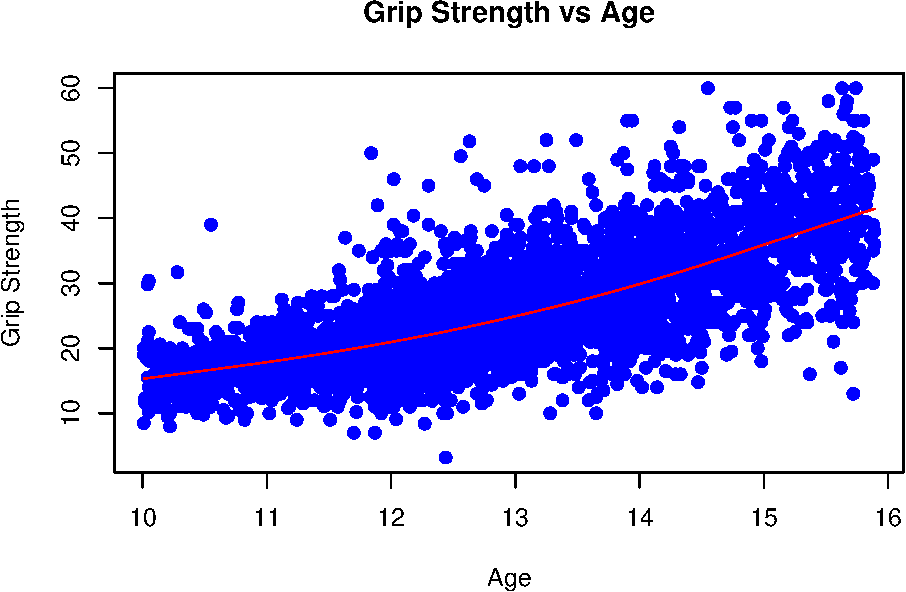
\includegraphics{assignment_q2_grip_files/figure-latex/unnamed-chunk-4-1.pdf}

\begin{Shaded}
\begin{Highlighting}[]
\CommentTok{\# Plot sample grip against age}
\FunctionTok{plot}\NormalTok{(grip\_sample}\SpecialCharTok{$}\NormalTok{age, grip\_sample}\SpecialCharTok{$}\NormalTok{grip,}
     \AttributeTok{xlab =} \StringTok{"Age"}\NormalTok{,}
     \AttributeTok{ylab =} \StringTok{"Grip Strength"}\NormalTok{,}
     \AttributeTok{main =} \StringTok{"Grip Strength vs Age"}\NormalTok{,}
     \AttributeTok{col =} \StringTok{"blue"}\NormalTok{,}
     \AttributeTok{pch =} \DecValTok{19}\NormalTok{)}

\CommentTok{\# Add a smooth line to highlight the trend}
\FunctionTok{lines}\NormalTok{(}\FunctionTok{smooth.spline}\NormalTok{(grip\_sample}\SpecialCharTok{$}\NormalTok{age, grip\_sample}\SpecialCharTok{$}\NormalTok{grip), }\AttributeTok{col =} \StringTok{"red"}\NormalTok{)}
\end{Highlighting}
\end{Shaded}

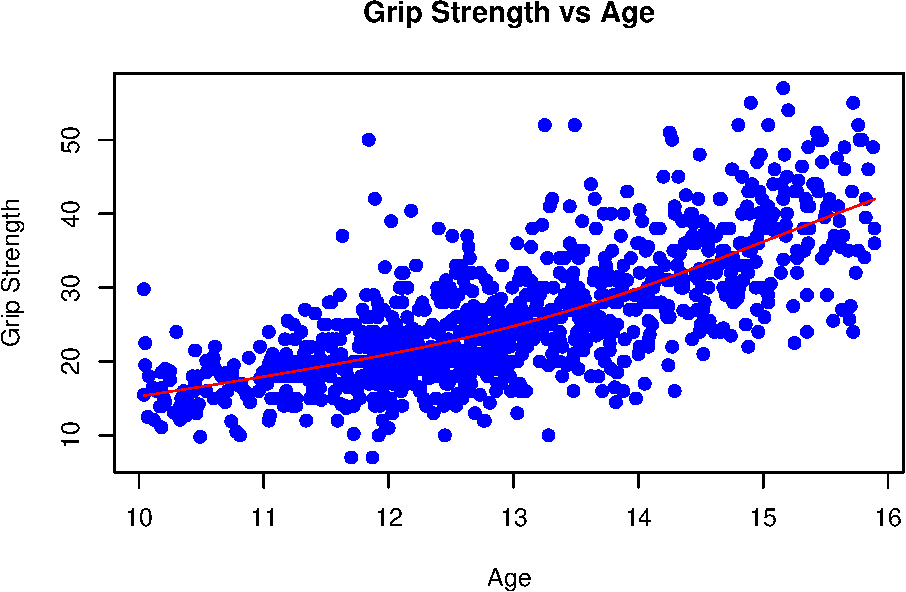
\includegraphics{assignment_q2_grip_files/figure-latex/unnamed-chunk-4-2.pdf}

Use the LMS method to fit the data.

\begin{Shaded}
\begin{Highlighting}[]
\CommentTok{\# Fit the model}
\NormalTok{gbccg }\OtherTok{\textless{}{-}} \FunctionTok{gamlss}\NormalTok{(grip }\SpecialCharTok{\textasciitilde{}} \FunctionTok{pb}\NormalTok{(age),}
                \AttributeTok{sigma.fo =} \SpecialCharTok{\textasciitilde{}} \FunctionTok{pb}\NormalTok{(age),}
                \AttributeTok{nu.fo =} \SpecialCharTok{\textasciitilde{}} \FunctionTok{pb}\NormalTok{(age),}
                \AttributeTok{data =}\NormalTok{ grip\_sample,}
                \AttributeTok{family =}\NormalTok{ BCCG)}
\end{Highlighting}
\end{Shaded}

\begin{verbatim}
## GAMLSS-RS iteration 1: Global Deviance = 6242.993 
## GAMLSS-RS iteration 2: Global Deviance = 6246.787 
## GAMLSS-RS iteration 3: Global Deviance = 6246.781 
## GAMLSS-RS iteration 4: Global Deviance = 6246.801 
## GAMLSS-RS iteration 5: Global Deviance = 6246.804 
## GAMLSS-RS iteration 6: Global Deviance = 6246.805
\end{verbatim}

\begin{Shaded}
\begin{Highlighting}[]
\CommentTok{\# Extract Effective Degrees of Freedom}
\NormalTok{edf\_gbccg }\OtherTok{\textless{}{-}} \FunctionTok{edfAll}\NormalTok{(gbccg)}
\end{Highlighting}
\end{Shaded}

Use the fitted values from the LMS model as starting values for fitting
the BCT and the BCPE distributions to the data

\begin{Shaded}
\begin{Highlighting}[]
\CommentTok{\# Fit the BCT model using gbccg as starting values}
\NormalTok{gbct }\OtherTok{\textless{}{-}} \FunctionTok{gamlss}\NormalTok{(grip }\SpecialCharTok{\textasciitilde{}} \FunctionTok{pb}\NormalTok{(age),}
               \AttributeTok{sigma.fo =} \SpecialCharTok{\textasciitilde{}} \FunctionTok{pb}\NormalTok{(age),}
               \AttributeTok{nu.fo =} \SpecialCharTok{\textasciitilde{}} \FunctionTok{pb}\NormalTok{(age),}
               \AttributeTok{tau.fo =} \SpecialCharTok{\textasciitilde{}} \FunctionTok{pb}\NormalTok{(age),}
               \AttributeTok{data =}\NormalTok{ grip\_sample,}
               \AttributeTok{family =}\NormalTok{ BCT,}
               \AttributeTok{start.from =}\NormalTok{ gbccg)}
\end{Highlighting}
\end{Shaded}

\begin{verbatim}
## GAMLSS-RS iteration 1: Global Deviance = 6243.64 
## GAMLSS-RS iteration 2: Global Deviance = 6241.875 
## GAMLSS-RS iteration 3: Global Deviance = 6241.464 
## GAMLSS-RS iteration 4: Global Deviance = 6241.311 
## GAMLSS-RS iteration 5: Global Deviance = 6241.251 
## GAMLSS-RS iteration 6: Global Deviance = 6241.225 
## GAMLSS-RS iteration 7: Global Deviance = 6241.215 
## GAMLSS-RS iteration 8: Global Deviance = 6241.208 
## GAMLSS-RS iteration 9: Global Deviance = 6241.206 
## GAMLSS-RS iteration 10: Global Deviance = 6241.205
\end{verbatim}

\begin{Shaded}
\begin{Highlighting}[]
\CommentTok{\# Fit the BCPE model using gbccg as starting values}
\NormalTok{gbcpe }\OtherTok{\textless{}{-}} \FunctionTok{gamlss}\NormalTok{(grip }\SpecialCharTok{\textasciitilde{}} \FunctionTok{pb}\NormalTok{(age),}
                \AttributeTok{sigma.fo =} \SpecialCharTok{\textasciitilde{}} \FunctionTok{pb}\NormalTok{(age),}
                \AttributeTok{nu.fo =} \SpecialCharTok{\textasciitilde{}} \FunctionTok{pb}\NormalTok{(age),}
                \AttributeTok{tau.fo =} \SpecialCharTok{\textasciitilde{}} \FunctionTok{pb}\NormalTok{(age),}
                \AttributeTok{data =}\NormalTok{ grip\_sample,}
                \AttributeTok{family =}\NormalTok{ BCPE,}
                \AttributeTok{start.from =}\NormalTok{ gbccg)}
\end{Highlighting}
\end{Shaded}

\begin{verbatim}
## GAMLSS-RS iteration 1: Global Deviance = 6241.603 
## GAMLSS-RS iteration 2: Global Deviance = 6241.32 
## GAMLSS-RS iteration 3: Global Deviance = 6241.293 
## GAMLSS-RS iteration 4: Global Deviance = 6241.292
\end{verbatim}

Effective degrees of freedom fitted for the parameters.

\begin{Shaded}
\begin{Highlighting}[]
\CommentTok{\# The EDF indicates the complexity of the model related to each parameter.}

\CommentTok{\# Extract EDF for BCT model}
\NormalTok{edf\_bct }\OtherTok{\textless{}{-}} \FunctionTok{edfAll}\NormalTok{(gbct)}

\CommentTok{\# Extract EDF for BCPE model}
\NormalTok{edf\_bcpe }\OtherTok{\textless{}{-}} \FunctionTok{edfAll}\NormalTok{(gbcpe)}

\CommentTok{\# Print the EDF for each model}
\FunctionTok{print}\NormalTok{(}\StringTok{"BCCG EDF"}\NormalTok{)}
\end{Highlighting}
\end{Shaded}

\begin{verbatim}
## [1] "BCCG EDF"
\end{verbatim}

\begin{Shaded}
\begin{Highlighting}[]
\FunctionTok{print}\NormalTok{(edf\_gbccg)}
\end{Highlighting}
\end{Shaded}

\begin{verbatim}
## $mu
## $mu$`pb(age)`
## [1] 4.713324
## 
## 
## $sigma
## $sigma$`pb(age)`
## [1] 3.319469
## 
## 
## $nu
## $nu$`pb(age)`
## [1] 2.000121
\end{verbatim}

\begin{Shaded}
\begin{Highlighting}[]
\FunctionTok{print}\NormalTok{(}\StringTok{"BCT EDF"}\NormalTok{)}
\end{Highlighting}
\end{Shaded}

\begin{verbatim}
## [1] "BCT EDF"
\end{verbatim}

\begin{Shaded}
\begin{Highlighting}[]
\FunctionTok{print}\NormalTok{(edf\_bct)}
\end{Highlighting}
\end{Shaded}

\begin{verbatim}
## $mu
## $mu$`pb(age)`
## [1] 4.733671
## 
## 
## $sigma
## $sigma$`pb(age)`
## [1] 3.444705
## 
## 
## $nu
## $nu$`pb(age)`
## [1] 2.000124
## 
## 
## $tau
## $tau$`pb(age)`
## [1] 2.000014
\end{verbatim}

\begin{Shaded}
\begin{Highlighting}[]
\FunctionTok{print}\NormalTok{(}\StringTok{"BCPE EDF"}\NormalTok{)}
\end{Highlighting}
\end{Shaded}

\begin{verbatim}
## [1] "BCPE EDF"
\end{verbatim}

\begin{Shaded}
\begin{Highlighting}[]
\FunctionTok{print}\NormalTok{(edf\_bcpe)}
\end{Highlighting}
\end{Shaded}

\begin{verbatim}
## $mu
## $mu$`pb(age)`
## [1] 4.727011
## 
## 
## $sigma
## $sigma$`pb(age)`
## [1] 3.350044
## 
## 
## $nu
## $nu$`pb(age)`
## [1] 2.000108
## 
## 
## $tau
## $tau$`pb(age)`
## [1] 2.000317
\end{verbatim}

\begin{Shaded}
\begin{Highlighting}[]
\FunctionTok{edfAll}\NormalTok{(gbcpe)}
\end{Highlighting}
\end{Shaded}

\begin{verbatim}
## $mu
## $mu$`pb(age)`
## [1] 4.727011
## 
## 
## $sigma
## $sigma$`pb(age)`
## [1] 3.350044
## 
## 
## $nu
## $nu$`pb(age)`
## [1] 2.000108
## 
## 
## $tau
## $tau$`pb(age)`
## [1] 2.000317
\end{verbatim}

GAIC to compare the three models.

\begin{Shaded}
\begin{Highlighting}[]
\CommentTok{\# Calculate GAIC for each model}
\NormalTok{gaic\_bccg }\OtherTok{\textless{}{-}} \FunctionTok{GAIC}\NormalTok{(gbccg)}
\NormalTok{gaic\_gbct }\OtherTok{\textless{}{-}} \FunctionTok{GAIC}\NormalTok{(gbct)}
\NormalTok{gaic\_gbcpe }\OtherTok{\textless{}{-}} \FunctionTok{GAIC}\NormalTok{(gbcpe)}

\CommentTok{\# Print the GAIC values}
\FunctionTok{print}\NormalTok{(}\FunctionTok{paste}\NormalTok{(}\StringTok{"GAIC for BCCG:"}\NormalTok{, gaic\_bccg))}
\end{Highlighting}
\end{Shaded}

\begin{verbatim}
## [1] "GAIC for BCCG: 6266.87079383024"
\end{verbatim}

\begin{Shaded}
\begin{Highlighting}[]
\FunctionTok{print}\NormalTok{(}\FunctionTok{paste}\NormalTok{(}\StringTok{"GAIC for BCT:"}\NormalTok{, gaic\_gbct))}
\end{Highlighting}
\end{Shaded}

\begin{verbatim}
## [1] "GAIC for BCT: 6265.56229903994"
\end{verbatim}

\begin{Shaded}
\begin{Highlighting}[]
\FunctionTok{print}\NormalTok{(}\FunctionTok{paste}\NormalTok{(}\StringTok{"GAIC for BCPE:"}\NormalTok{, gaic\_gbcpe))}
\end{Highlighting}
\end{Shaded}

\begin{verbatim}
## [1] "GAIC for BCPE: 6265.44681092804"
\end{verbatim}

Plot the fitted parameters for the fitted models

\begin{Shaded}
\begin{Highlighting}[]
\CommentTok{\# \textquotesingle{}gbccg\textquotesingle{} and \textquotesingle{}gbct\textquotesingle{} are fitted models}
\FunctionTok{fittedPlot}\NormalTok{(gbccg, gbct, }\AttributeTok{x=}\NormalTok{grip\_sample}\SpecialCharTok{$}\NormalTok{age)}
\end{Highlighting}
\end{Shaded}

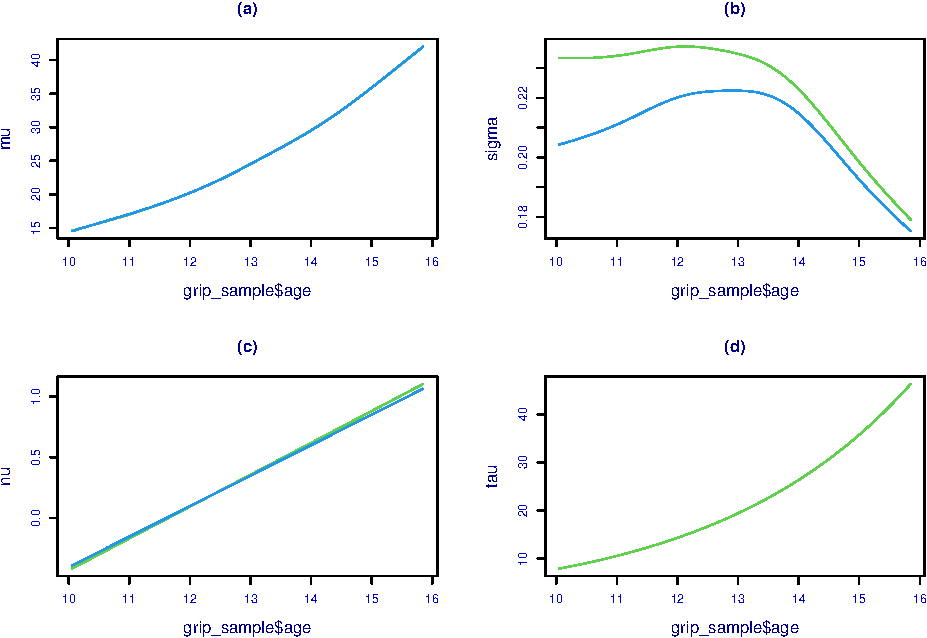
\includegraphics{assignment_q2_grip_files/figure-latex/unnamed-chunk-10-1.pdf}

\begin{Shaded}
\begin{Highlighting}[]
\CommentTok{\# Calculate fitted values or centiles for each model across a range of ages}
\NormalTok{age\_seq }\OtherTok{\textless{}{-}} \FunctionTok{seq}\NormalTok{(}\FunctionTok{min}\NormalTok{(grip\_sample}\SpecialCharTok{$}\NormalTok{age), }\FunctionTok{max}\NormalTok{(grip\_sample}\SpecialCharTok{$}\NormalTok{age), }\AttributeTok{length.out =} \DecValTok{100}\NormalTok{)}

\CommentTok{\# For BCCG Model}
\NormalTok{fitted\_bccg }\OtherTok{\textless{}{-}} \FunctionTok{predict}\NormalTok{(gbccg, }\AttributeTok{newdata=}\FunctionTok{data.frame}\NormalTok{(}\AttributeTok{age=}\NormalTok{age\_seq), }\AttributeTok{type=}\StringTok{"response"}\NormalTok{)}
\end{Highlighting}
\end{Shaded}

\begin{verbatim}
## new prediction
\end{verbatim}

\begin{Shaded}
\begin{Highlighting}[]
\CommentTok{\# For BCT Model}
\NormalTok{fitted\_gbct }\OtherTok{\textless{}{-}} \FunctionTok{predict}\NormalTok{(gbct, }\AttributeTok{newdata=}\FunctionTok{data.frame}\NormalTok{(}\AttributeTok{age=}\NormalTok{age\_seq), }\AttributeTok{type=}\StringTok{"response"}\NormalTok{)}
\end{Highlighting}
\end{Shaded}

\begin{verbatim}
## new prediction
\end{verbatim}

\begin{Shaded}
\begin{Highlighting}[]
\CommentTok{\# Plotting}
\FunctionTok{plot}\NormalTok{(age\_seq, fitted\_bccg, }\AttributeTok{type=}\StringTok{\textquotesingle{}l\textquotesingle{}}\NormalTok{, }\AttributeTok{col=}\StringTok{\textquotesingle{}blue\textquotesingle{}}\NormalTok{, }\AttributeTok{ylim=}\FunctionTok{range}\NormalTok{(}\FunctionTok{c}\NormalTok{(fitted\_bccg, fitted\_gbct)),}
     \AttributeTok{xlab=}\StringTok{\textquotesingle{}Age\textquotesingle{}}\NormalTok{, }\AttributeTok{ylab=}\StringTok{\textquotesingle{}Fitted Grip Strength\textquotesingle{}}\NormalTok{, }\AttributeTok{main=}\StringTok{\textquotesingle{}Fitted Models Comparison\textquotesingle{}}\NormalTok{)}
\FunctionTok{lines}\NormalTok{(age\_seq, fitted\_gbct, }\AttributeTok{col=}\StringTok{\textquotesingle{}red\textquotesingle{}}\NormalTok{)}

\CommentTok{\# Adding a legend}
\FunctionTok{legend}\NormalTok{(}\StringTok{"topright"}\NormalTok{, }\AttributeTok{legend=}\FunctionTok{c}\NormalTok{(}\StringTok{"BCCG"}\NormalTok{, }\StringTok{"BCT"}\NormalTok{), }\AttributeTok{col=}\FunctionTok{c}\NormalTok{(}\StringTok{"blue"}\NormalTok{, }\StringTok{"red"}\NormalTok{), }\AttributeTok{lty=}\DecValTok{1}\NormalTok{, }\AttributeTok{cex=}\FloatTok{0.8}\NormalTok{)}
\end{Highlighting}
\end{Shaded}

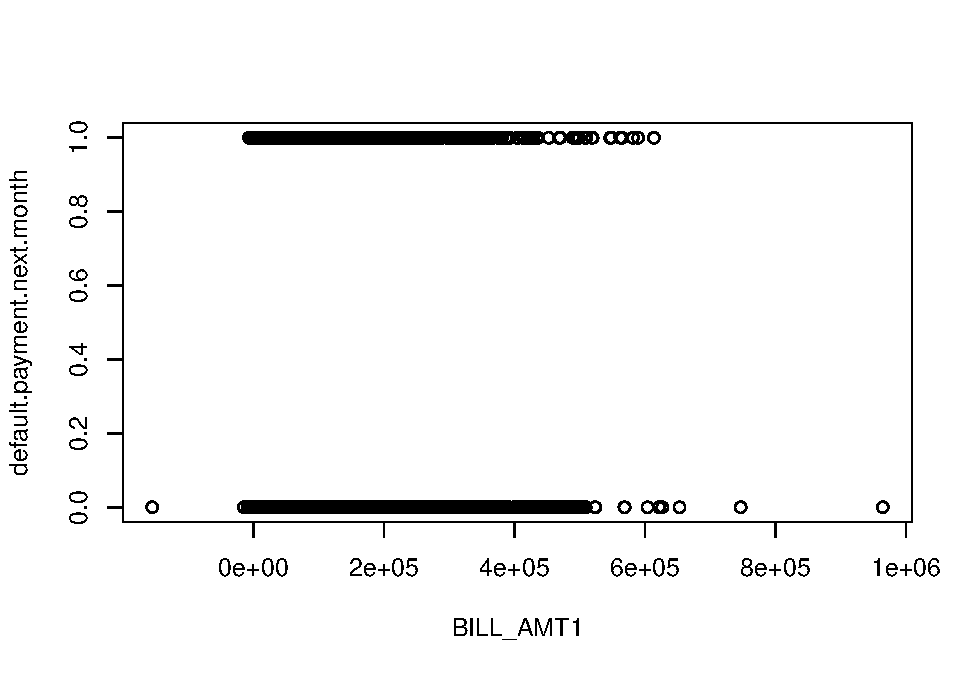
\includegraphics{assignment_q2_grip_files/figure-latex/unnamed-chunk-10-2.pdf}

Centile plot for the fitted models.

\begin{Shaded}
\begin{Highlighting}[]
\FunctionTok{centilesTwo}\NormalTok{(gbccg, }\DecValTok{10}\SpecialCharTok{:}\DecValTok{16}\NormalTok{, }\FunctionTok{seq}\NormalTok{(}\DecValTok{15}\NormalTok{, }\DecValTok{40}\NormalTok{, }\DecValTok{5}\NormalTok{), age,  grip, }\AttributeTok{cent=}\FloatTok{0.05}\NormalTok{, }\AttributeTok{dist=}\NormalTok{.}\DecValTok{1}\NormalTok{, }\AttributeTok{xlab=}\StringTok{"age"}\NormalTok{, }\AttributeTok{ylab=}\StringTok{\textquotesingle{}grip\textquotesingle{}}\NormalTok{)}
\end{Highlighting}
\end{Shaded}

\begin{verbatim}
## new prediction 
## new prediction 
## new prediction
\end{verbatim}

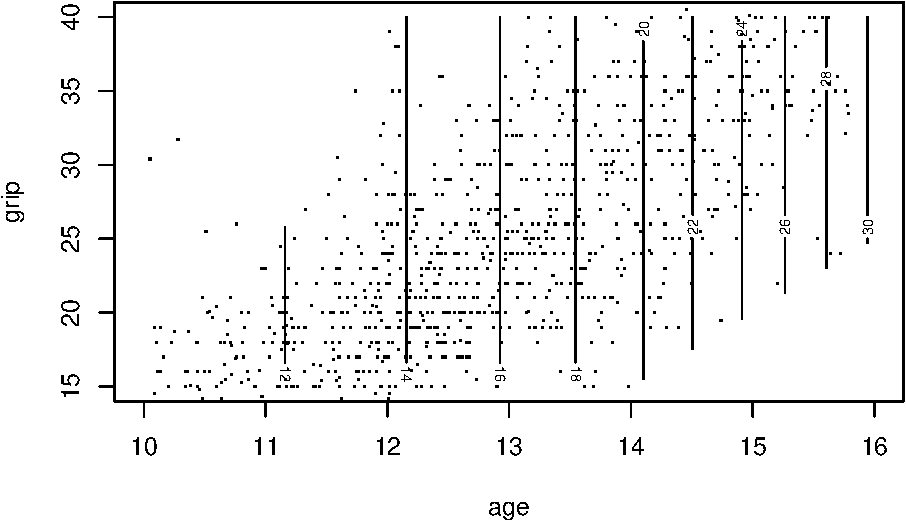
\includegraphics{assignment_q2_grip_files/figure-latex/unnamed-chunk-11-1.pdf}

\begin{Shaded}
\begin{Highlighting}[]
\FunctionTok{centiles}\NormalTok{(gbccg, }\AttributeTok{xvar=}\NormalTok{grip\_sample}\SpecialCharTok{$}\NormalTok{age, }\AttributeTok{col=}\StringTok{"blue"}\NormalTok{, }\AttributeTok{lty =} \DecValTok{3}\NormalTok{, }\AttributeTok{cent=}\FunctionTok{c}\NormalTok{(}\FloatTok{0.1}\NormalTok{, }\FloatTok{0.4}\NormalTok{, }\DecValTok{2}\NormalTok{,}\DecValTok{10}\NormalTok{, }\DecValTok{25}\NormalTok{, }\DecValTok{50}\NormalTok{,}\DecValTok{75}\NormalTok{,}\DecValTok{90}\NormalTok{,}\DecValTok{98}\NormalTok{,}\FloatTok{99.6}\NormalTok{, }\FloatTok{99.9}\NormalTok{), }\AttributeTok{ylab=}\StringTok{"grip"}\NormalTok{, }\AttributeTok{xlab=}\StringTok{"age"}\NormalTok{)}
\end{Highlighting}
\end{Shaded}

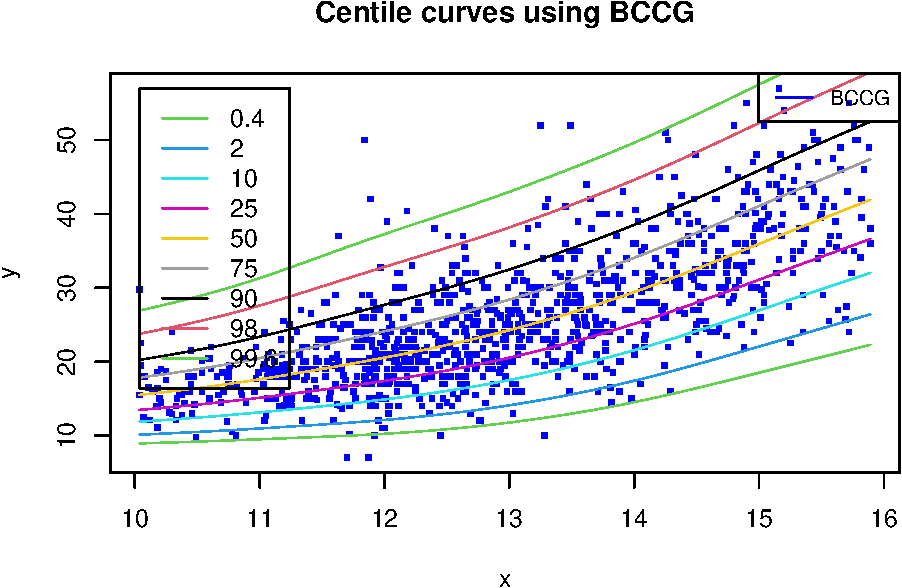
\includegraphics{assignment_q2_grip_files/figure-latex/unnamed-chunk-11-2.pdf}

\begin{verbatim}
## % of cases below  0.1 centile is  0.2 
## % of cases below  0.4 centile is  0.7 
## % of cases below  2 centile is  2.3 
## % of cases below  10 centile is  8.7 
## % of cases below  25 centile is  24.8 
## % of cases below  50 centile is  49.9 
## % of cases below  75 centile is  75 
## % of cases below  90 centile is  91.2 
## % of cases below  98 centile is  97.9 
## % of cases below  99.6 centile is  99.1 
## % of cases below  99.9 centile is  99.7
\end{verbatim}

\begin{Shaded}
\begin{Highlighting}[]
\CommentTok{\# Plot centiles for BCCG model}
\FunctionTok{plot}\NormalTok{(grip\_sample}\SpecialCharTok{$}\NormalTok{age, grip\_sample}\SpecialCharTok{$}\NormalTok{grip, }\AttributeTok{col=}\StringTok{"gray90"}\NormalTok{, }\AttributeTok{main=}\StringTok{"Centile Comparison"}\NormalTok{, }\AttributeTok{xlab=}\StringTok{"Age"}\NormalTok{, }\AttributeTok{ylab=}\StringTok{"Grip Strength"}\NormalTok{)}
\end{Highlighting}
\end{Shaded}

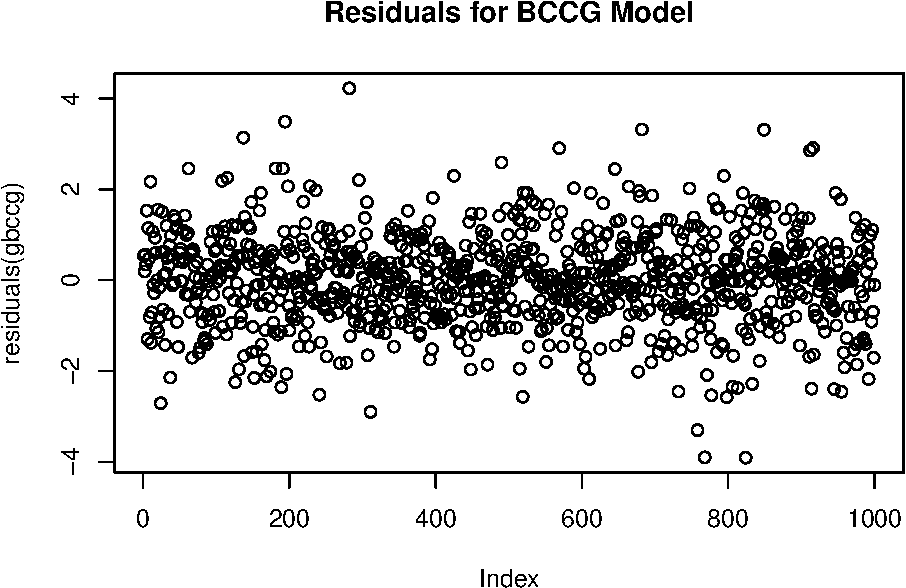
\includegraphics{assignment_q2_grip_files/figure-latex/unnamed-chunk-12-1.pdf}

\begin{Shaded}
\begin{Highlighting}[]
\CommentTok{\# Add centiles for BCT model to the existing plot}
\FunctionTok{centiles}\NormalTok{(gbct, }\AttributeTok{xvar =}\NormalTok{ grip\_sample}\SpecialCharTok{$}\NormalTok{age, }\AttributeTok{col =} \StringTok{"blue"}\NormalTok{, }\AttributeTok{lty =} \DecValTok{2}\NormalTok{, }\AttributeTok{cent=}\FunctionTok{c}\NormalTok{(}\FloatTok{0.1}\NormalTok{, }\FloatTok{0.4}\NormalTok{, }\DecValTok{2}\NormalTok{,}\DecValTok{10}\NormalTok{, }\DecValTok{25}\NormalTok{, }\DecValTok{50}\NormalTok{,}\DecValTok{75}\NormalTok{,}\DecValTok{90}\NormalTok{,}\DecValTok{98}\NormalTok{,}\FloatTok{99.6}\NormalTok{, }\FloatTok{99.9}\NormalTok{), }\AttributeTok{ylab=}\StringTok{"grip"}\NormalTok{, }\AttributeTok{xlab=}\StringTok{"age"}\NormalTok{)}
\end{Highlighting}
\end{Shaded}

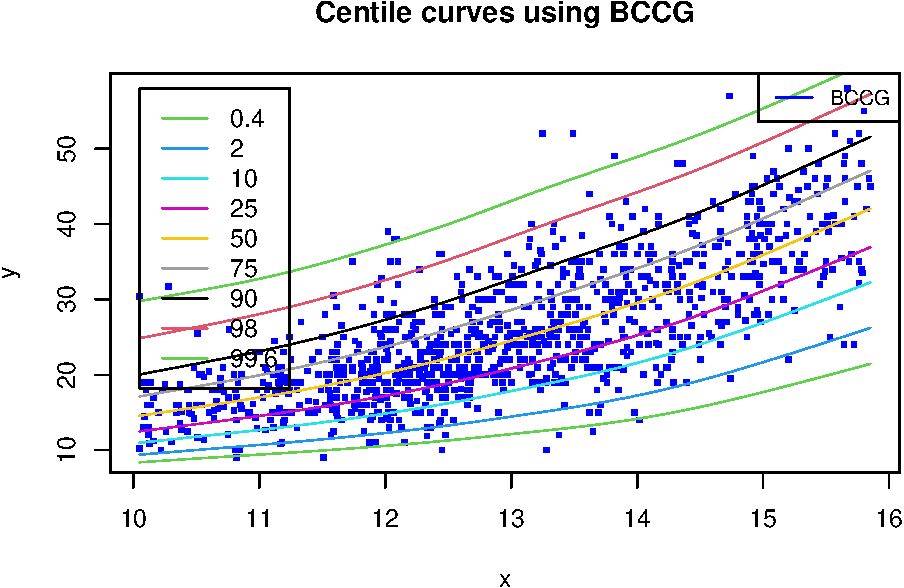
\includegraphics{assignment_q2_grip_files/figure-latex/unnamed-chunk-12-2.pdf}

\begin{verbatim}
## % of cases below  0.1 centile is  0.1 
## % of cases below  0.4 centile is  0.5 
## % of cases below  2 centile is  2.3 
## % of cases below  10 centile is  9.3 
## % of cases below  25 centile is  25.3 
## % of cases below  50 centile is  50 
## % of cases below  75 centile is  74.4 
## % of cases below  90 centile is  90.4 
## % of cases below  98 centile is  98 
## % of cases below  99.6 centile is  99.6 
## % of cases below  99.9 centile is  99.8
\end{verbatim}

\begin{Shaded}
\begin{Highlighting}[]
\FunctionTok{centiles}\NormalTok{(gbcpe, }\AttributeTok{xvar =}\NormalTok{ grip\_sample}\SpecialCharTok{$}\NormalTok{age, }\AttributeTok{col =} \StringTok{"blue"}\NormalTok{, }\AttributeTok{lty =} \DecValTok{1}\NormalTok{, }\AttributeTok{cent=}\FunctionTok{c}\NormalTok{(}\FloatTok{0.1}\NormalTok{, }\FloatTok{0.4}\NormalTok{, }\DecValTok{2}\NormalTok{,}\DecValTok{10}\NormalTok{, }\DecValTok{25}\NormalTok{, }\DecValTok{50}\NormalTok{,}\DecValTok{75}\NormalTok{,}\DecValTok{90}\NormalTok{,}\DecValTok{98}\NormalTok{,}\FloatTok{99.6}\NormalTok{, }\FloatTok{99.9}\NormalTok{), }\AttributeTok{ylab=}\StringTok{"grip"}\NormalTok{, }\AttributeTok{xlab=}\StringTok{"age"}\NormalTok{)}
\end{Highlighting}
\end{Shaded}

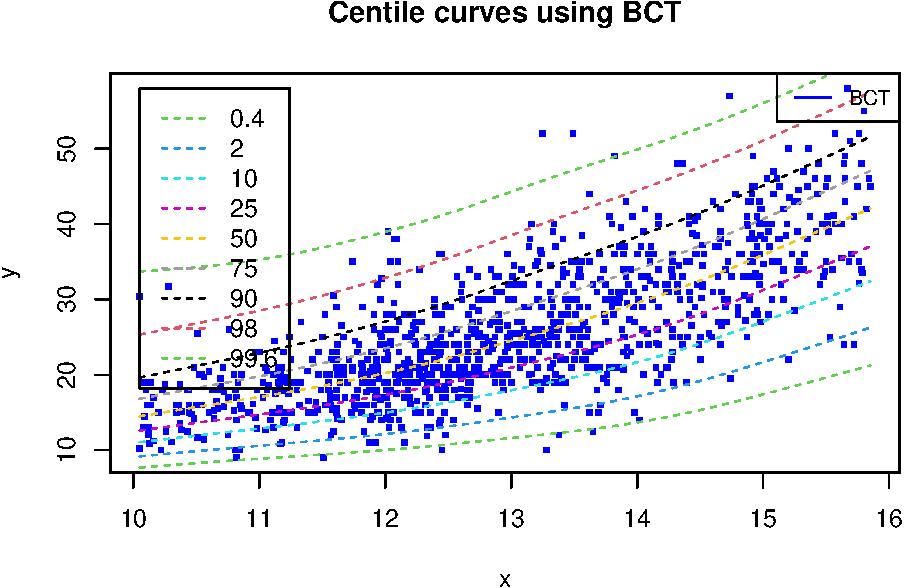
\includegraphics{assignment_q2_grip_files/figure-latex/unnamed-chunk-12-3.pdf}

\begin{verbatim}
## % of cases below  0.1 centile is  0.1 
## % of cases below  0.4 centile is  0.6 
## % of cases below  2 centile is  2.2 
## % of cases below  10 centile is  9 
## % of cases below  25 centile is  25.6 
## % of cases below  50 centile is  49.8 
## % of cases below  75 centile is  74.3 
## % of cases below  90 centile is  90.7 
## % of cases below  98 centile is  98.1 
## % of cases below  99.6 centile is  99.5 
## % of cases below  99.9 centile is  99.7
\end{verbatim}

\begin{Shaded}
\begin{Highlighting}[]
\CommentTok{\#legend("topright", legend=c("BCCG"), col=c("blue"), lty=1, cex=0.8)}

\CommentTok{\# Update the legend to include BCT}
\CommentTok{\#legend("topright", legend=c("BCCG"), col=c("blue"), lty=1:2, cex=0.8)}
\end{Highlighting}
\end{Shaded}

Residuals from the fitted models:

\begin{Shaded}
\begin{Highlighting}[]
\CommentTok{\# For BCCG Model}
\FunctionTok{plot}\NormalTok{(}\FunctionTok{residuals}\NormalTok{(gbccg), }\AttributeTok{main=}\StringTok{"Residuals for BCCG Model"}\NormalTok{)}
\end{Highlighting}
\end{Shaded}

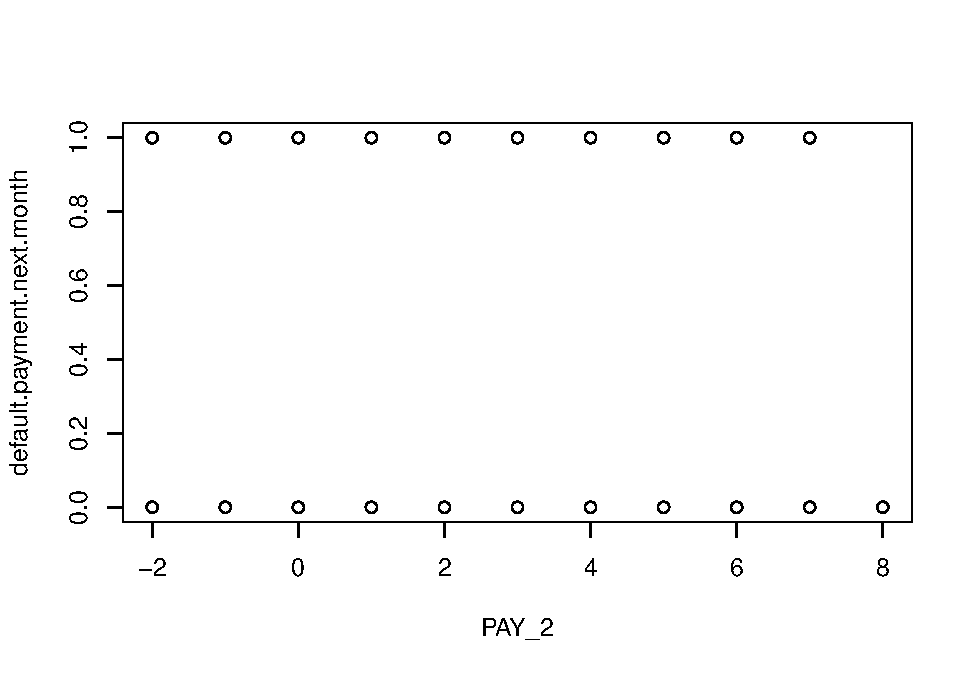
\includegraphics{assignment_q2_grip_files/figure-latex/unnamed-chunk-13-1.pdf}

\begin{Shaded}
\begin{Highlighting}[]
\CommentTok{\# For BCT Model}
\FunctionTok{plot}\NormalTok{(}\FunctionTok{residuals}\NormalTok{(gbct), }\AttributeTok{main=}\StringTok{"Residuals for BCT Model"}\NormalTok{)}
\end{Highlighting}
\end{Shaded}

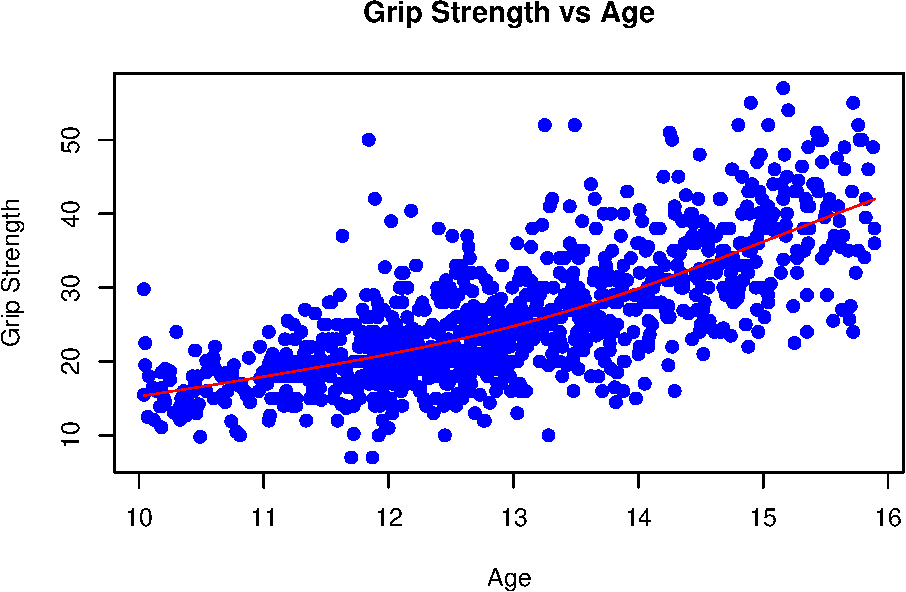
\includegraphics{assignment_q2_grip_files/figure-latex/unnamed-chunk-13-2.pdf}

\begin{Shaded}
\begin{Highlighting}[]
\CommentTok{\# For BCCG Model}
\FunctionTok{wp}\NormalTok{(gbccg, }\AttributeTok{main=}\StringTok{"Worm Plot for BCCG Model"}\NormalTok{)}
\end{Highlighting}
\end{Shaded}

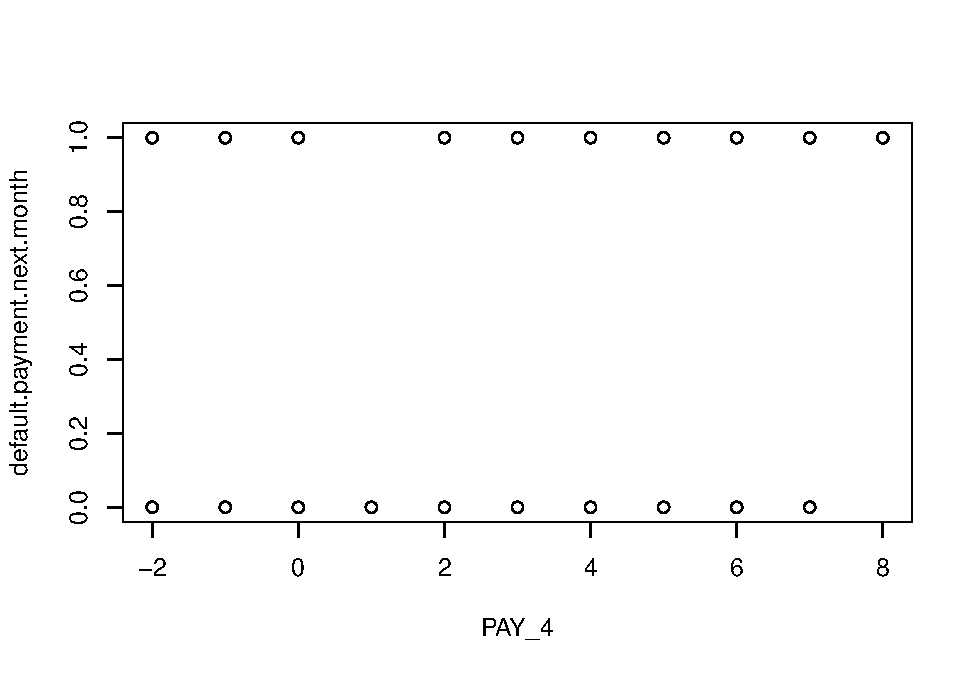
\includegraphics{assignment_q2_grip_files/figure-latex/unnamed-chunk-13-3.pdf}

\begin{Shaded}
\begin{Highlighting}[]
\CommentTok{\# For BCT Model}
\FunctionTok{wp}\NormalTok{(gbct, }\AttributeTok{main=}\StringTok{"Worm Plot for BCT Model"}\NormalTok{)}
\end{Highlighting}
\end{Shaded}

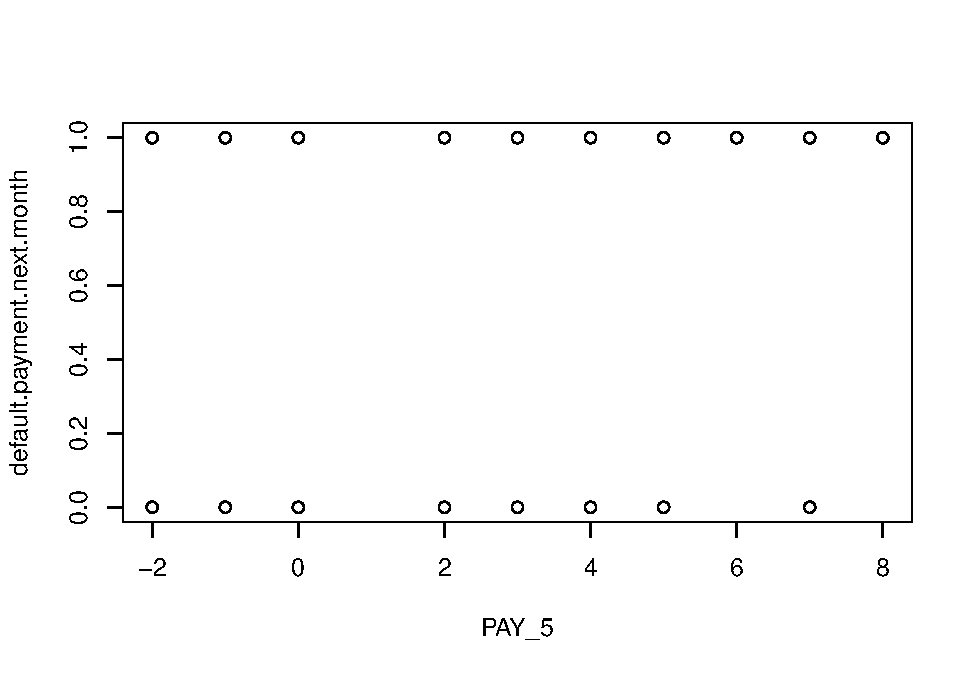
\includegraphics{assignment_q2_grip_files/figure-latex/unnamed-chunk-13-4.pdf}

\begin{Shaded}
\begin{Highlighting}[]
\CommentTok{\# For BCPE Model}
\FunctionTok{wp}\NormalTok{(gbcpe, }\AttributeTok{main=}\StringTok{"Worm Plot for BCPE Model"}\NormalTok{)}
\end{Highlighting}
\end{Shaded}

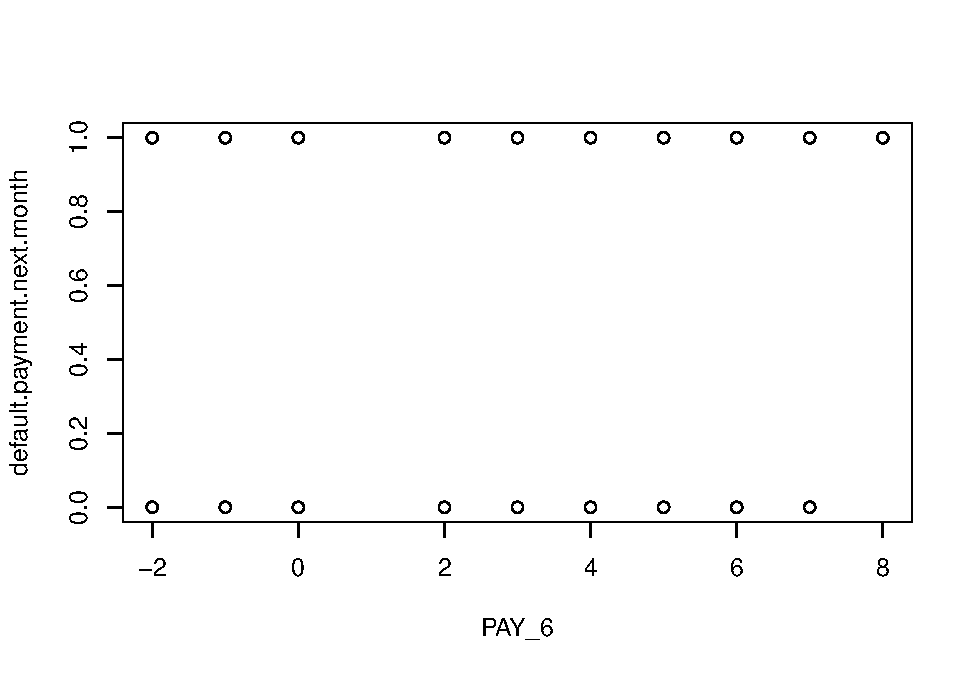
\includegraphics{assignment_q2_grip_files/figure-latex/unnamed-chunk-13-5.pdf}

\begin{Shaded}
\begin{Highlighting}[]
\CommentTok{\# For BCCG Model}
\NormalTok{qstats\_bccg }\OtherTok{\textless{}{-}} \FunctionTok{Q.stats}\NormalTok{(gbccg)}
\end{Highlighting}
\end{Shaded}

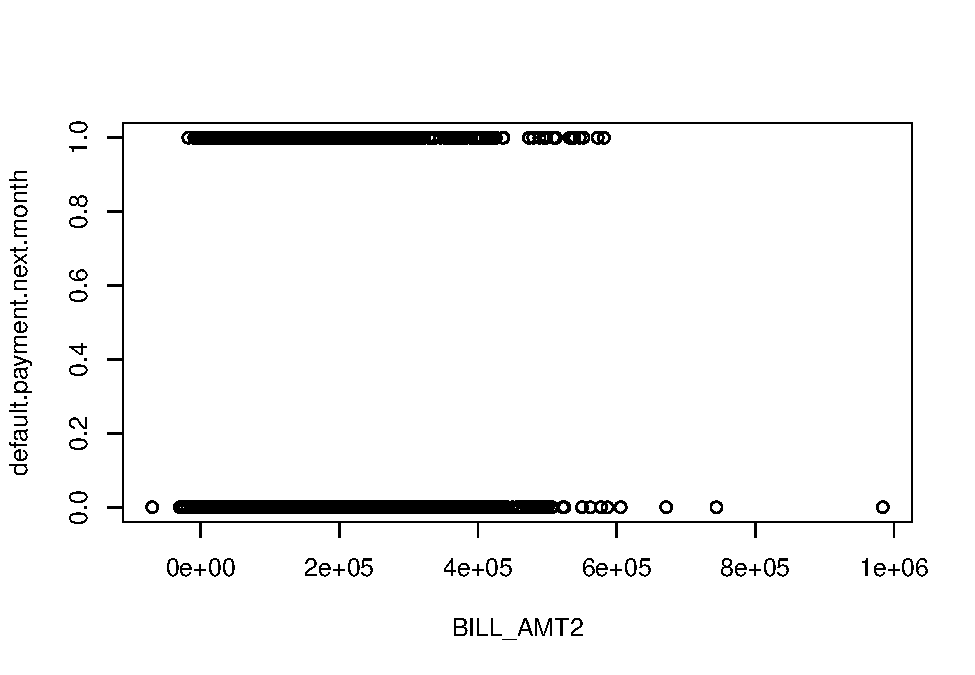
\includegraphics{assignment_q2_grip_files/figure-latex/unnamed-chunk-13-6.pdf}

\begin{Shaded}
\begin{Highlighting}[]
\FunctionTok{print}\NormalTok{(qstats\_bccg)}
\end{Highlighting}
\end{Shaded}

\begin{verbatim}
##                             Z1          Z2          Z3          Z4   AgostinoK2
##    0.5 to  100.5  -0.203907433  1.85395837 -1.96268227  0.75852485  4.427481630
##  100.5 to  200.5   2.402287804  0.28062802 -0.85776506 -2.79366506  8.540325397
##  200.5 to  300.5   0.871410159 -1.19936605  1.04028580  1.20345279  2.530493158
##  300.5 to  400.5   0.215184771 -1.49021285  1.85291013  2.70760397 10.764395207
##  400.5 to  500.5  -1.531442363 -2.15310227 -0.41383582  1.19895473  1.608752543
##  500.5 to  600.5   0.037281474 -0.06330455  0.56132156  0.86459185  1.062600958
##  600.5 to  700.5   0.416330909  1.38978751 -0.16687341  0.62308483  0.416081434
##  700.5 to  800.5  -0.930585700  0.51356221  1.05915525  1.26446329  2.720677240
##  800.5 to  900.5  -1.306755289  0.99110231  0.31603114  1.05594507  1.214895675
##  900.5 to 1000.5  -0.005296923 -1.25765363  0.08189189 -0.04731519  0.008945009
## TOTAL Q stats     11.711889316 16.57421573 10.84593361 22.44871464 33.294648249
## df for Q stats     5.286675988  7.84026565  7.99987911 10.00000000 17.999879110
## p-val for Q stats  0.046334806  0.03214421  0.21057399  0.01297493  0.015370373
##                      N
##    0.5 to  100.5   100
##  100.5 to  200.5   100
##  200.5 to  300.5   100
##  300.5 to  400.5   100
##  400.5 to  500.5   100
##  500.5 to  600.5   100
##  600.5 to  700.5   100
##  700.5 to  800.5   100
##  800.5 to  900.5   100
##  900.5 to 1000.5   100
## TOTAL Q stats     1000
## df for Q stats       0
## p-val for Q stats    0
\end{verbatim}

\begin{Shaded}
\begin{Highlighting}[]
\CommentTok{\# For BCT Model}
\NormalTok{qstats\_bct }\OtherTok{\textless{}{-}} \FunctionTok{Q.stats}\NormalTok{(gbct)}
\end{Highlighting}
\end{Shaded}

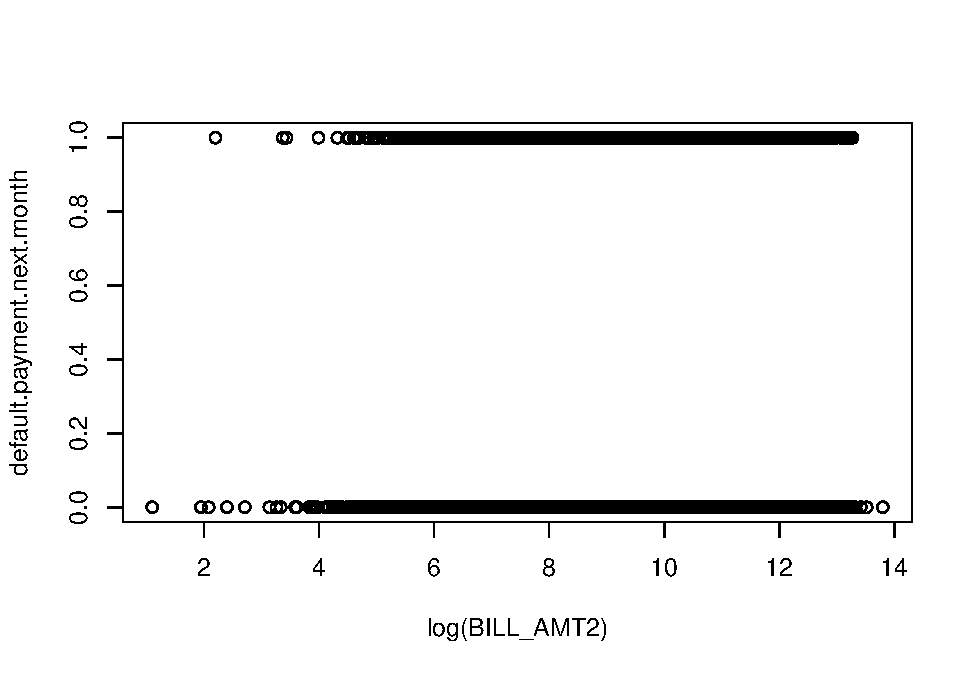
\includegraphics{assignment_q2_grip_files/figure-latex/unnamed-chunk-13-7.pdf}

\begin{Shaded}
\begin{Highlighting}[]
\FunctionTok{print}\NormalTok{(qstats\_bct)}
\end{Highlighting}
\end{Shaded}

\begin{verbatim}
##                             Z1          Z2         Z3          Z4  AgostinoK2
##    0.5 to  100.5  -0.150324437  1.75960447 -1.6292108  0.11704128  2.66802637
##  100.5 to  200.5   2.440492979  0.46954000 -0.9804560 -3.29497276 11.81813938
##  200.5 to  300.5   0.842962204 -1.08562505  0.5829998  0.33028150  0.44897466
##  300.5 to  400.5   0.170958501 -1.54178728  1.3770034  2.20209601  6.74536534
##  400.5 to  500.5  -1.523487794 -2.03988375  0.1163577  0.18062149  0.04616323
##  500.5 to  600.5   0.008605278 -0.02454827  0.3727182  0.31449406  0.23782540
##  600.5 to  700.5   0.440857942  1.23288881 -0.1201984  0.04439974  0.01641898
##  700.5 to  800.5  -0.937084732  0.46479961  0.8224300  0.44323903  0.87285192
##  800.5 to  900.5  -1.325056094  0.82985742  0.2824048  0.30526034  0.17293634
##  900.5 to 1000.5  -0.019382405 -1.11202793  0.0777290 -0.47198845  0.22881489
## TOTAL Q stats     11.868137464 14.69541676  6.7807399 16.47477665 23.25551652
## df for Q stats     5.266329280  7.77764748  7.9998764  7.99998585 15.99986227
## p-val for Q stats  0.043121921  0.05898312  0.5604506  0.03606707  0.10706852
##                      N
##    0.5 to  100.5   100
##  100.5 to  200.5   100
##  200.5 to  300.5   100
##  300.5 to  400.5   100
##  400.5 to  500.5   100
##  500.5 to  600.5   100
##  600.5 to  700.5   100
##  700.5 to  800.5   100
##  800.5 to  900.5   100
##  900.5 to 1000.5   100
## TOTAL Q stats     1000
## df for Q stats       0
## p-val for Q stats    0
\end{verbatim}

\begin{Shaded}
\begin{Highlighting}[]
\CommentTok{\# For BCPE Model}
\NormalTok{qstats\_bcpe }\OtherTok{\textless{}{-}} \FunctionTok{Q.stats}\NormalTok{(gbcpe)}
\end{Highlighting}
\end{Shaded}

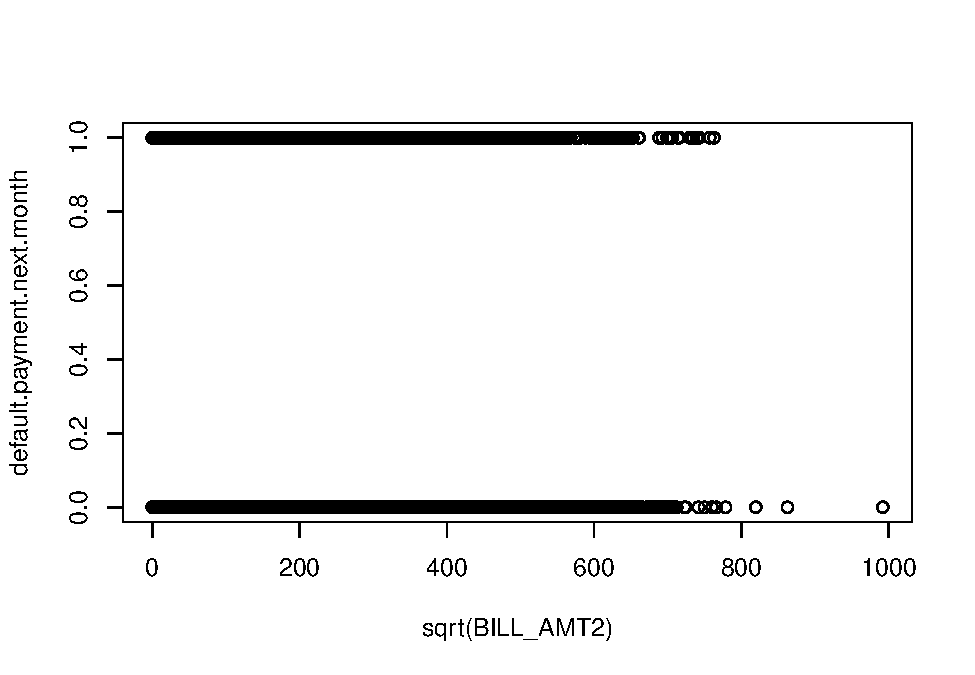
\includegraphics{assignment_q2_grip_files/figure-latex/unnamed-chunk-13-8.pdf}

\begin{Shaded}
\begin{Highlighting}[]
\FunctionTok{print}\NormalTok{(qstats\_bcpe)}
\end{Highlighting}
\end{Shaded}

\begin{verbatim}
##                              Z1          Z2          Z3          Z4  AgostinoK2
##    0.5 to  100.5  -0.2076165280  1.79549548 -1.74717054  0.28417899  3.13336258
##  100.5 to  200.5   2.4413036875  0.42720896 -0.97258731 -3.22067026 11.31864300
##  200.5 to  300.5   0.8360026267 -1.07355106  0.75752981  0.64999646  0.99634680
##  300.5 to  400.5   0.1897996768 -1.41809611  1.55669650  2.40094078  8.18782063
##  400.5 to  500.5  -1.5194876588 -2.06491214  0.01840007  0.28333747  0.08061869
##  500.5 to  600.5   0.0008666567 -0.04259841  0.34741633  0.39960296  0.28038063
##  600.5 to  700.5   0.4731497287  1.21316309 -0.11736924  0.14047244  0.03350804
##  700.5 to  800.5  -0.9122907238  0.47061393  0.94111416  0.74302772  1.43778605
##  800.5 to  900.5  -1.3411558367  0.79612461  0.30569504  0.36287822  0.22513006
##  900.5 to 1000.5  -0.0262868019 -1.17113674  0.06714718 -0.50253769  0.25705287
## TOTAL Q stats     11.9023711277 14.53411457  8.11415263 17.83649674 25.95064936
## df for Q stats     5.2729887486  7.82497824  7.99989176  7.99968292 15.99957467
## p-val for Q stats  0.0427286759  0.06359555  0.42238866  0.02248246  0.05471882
##                      N
##    0.5 to  100.5   100
##  100.5 to  200.5   100
##  200.5 to  300.5   100
##  300.5 to  400.5   100
##  400.5 to  500.5   100
##  500.5 to  600.5   100
##  600.5 to  700.5   100
##  700.5 to  800.5   100
##  800.5 to  900.5   100
##  900.5 to 1000.5   100
## TOTAL Q stats     1000
## df for Q stats       0
## p-val for Q stats    0
\end{verbatim}

\end{document}
